\documentclass[pdf,9pt]{beamer}
\usepackage{listings,graphicx,verbatimbox,hyperref}
\usepackage{hyperref}
\usepackage{bibentry}
\usepackage[customcolors,shade]{hf-tikz}
\newcommand{\N}{\mathbb{N}}
\newcommand{\Z}{\mathbb{Z}}
\newcommand{\Q}{\mathbb{Q}}
\newcommand{\R}{\mathbb{R}}
\newcommand{\C}{\mathbb{C}}

\newcommand{\norm}[1]{\left\lVert#1\right\rVert}
\newcommand{\ceil}[1]{\lceil#1\rceil}
\newcommand{\ov}{\overline}
\newcommand{\cleq}{\preccurlyeq}
\newcommand{\cgeq}{\succcurlyeq}
\newcommand{\bdy}{\textbf{\text{Bdy}}}
\newcommand{\trace}{\text{trace}}
\newcommand{\dom}{\textbf{dom}}
\newcommand{\expec}{\mathbb{E}}
\newcommand{\bigO}{\mathcal{O}}
\newcommand{\tr}{\text{tr}}
\newcommand{\<}{\langle}
\renewcommand{\>}{\rangle}
\newcommand*\oldmacro{}%
\let\oldmacro\insertshorttitle%
% \renewcommand*\insertshorttitle{%
%   \oldmacro\hfill%
%   \insertframenumber\,/\,\inserttotalframenumber}
\DeclareMathOperator*{\argmax}{arg\,max}
\DeclareMathOperator*{\argmin}{arg\,min}

% use the below command to restart numbering in an enumeration, using alphabetics
% \setbeamertemplate{enumerate item}{(\alph{enumi})}
% \setbeamertemplate{enumerate subitem}{(\roman{enumii})}
%\setbeamertemplate{navigation symbols}{}

\usetheme{Warsaw}
\setbeamertemplate{footline}
{
  \leavevmode%
  \hbox{%
  \begin{beamercolorbox}[wd=.3\paperwidth,ht=2.25ex,dp=1ex,center]{author in head/foot}%
    \usebeamerfont{author in head/foot}\insertshortauthor
  \end{beamercolorbox}%
  \begin{beamercolorbox}[wd=.7\paperwidth,ht=2.25ex,dp=1ex,center]{title in head/foot}%
    \usebeamerfont{title in head/foot}\insertshorttitle\hspace*{3em}
    \insertframenumber{} / \inserttotalframenumber\hspace*{1ex}
  \end{beamercolorbox}}%
  \vskip0pt%
}
% \setbeamertemplate{footline}[frame number]
\usepackage{biblatex}
\addbibresource{tetrad.bib}
\bibliography{tetrad}
\usepackage{caption}
\title{Feb 6 update}
%\author[cmhyett@math.arizona.edu]{Criston Hyett \inst{1}\inst{2} \and Michael Chertkov \inst{1} \and Yifeng Tian \inst{2} \and Daniel Livescu \inst{2} \and Misha Stepanov \inst{1} \and Michael Woodward \inst{1}\inst{2} \and Chris Fryer \inst{2}}

\graphicspath{{./figs/}}

\begin{document}

%%%%%%%%%%%%%%%%%%%%%%%%%%%%%%%%%%%%%%%%%%%%%%%%%%%%%%%%%%%%%%%%%%%%%%%%%%%%% 
\begin{frame}{Feb 6 Update}
  \begin{exampleblock}{Work Completed}
    \begin{itemize}
    \item Check temporal correlations of invariants and pressure hessian at $Re \approx 450$.
    \item Request high $Re$ data
    \item Check invariant distributions for high $Re$, compare variances to $Re = 240$
    \end{itemize}
  \end{exampleblock}

  \begin{block}{Work In Progress}
    \begin{itemize}
    \item Generalization over Reynolds number
      \begin{itemize}
      \item Re-run training at $Re = 430$
      \end{itemize}
    \item Benefits of reduced description      
      \begin{itemize}
      \item Posteriori tests for $Re = 240,430$ - more stable?
      \end{itemize}
    \item Explanation
      \begin{itemize}
      \item Can $\lambda_{3,4,5}$ be expressed in terms of $\lambda_{1,2}$?
      \item PDFs of eigenvalues of $W$ and $S$
      \end{itemize}
    
    \end{itemize}
  \end{block}
  
\end{frame}
%%%%%%%%%%%%%%%%%%%%%%%%%%%%%%%%%%%%%%%%%%%%%%%%%%%%%%%%%%%%%%%%%%%%%%%%%%%%%

%%%%%%%%%%%%%%%%%%%%%%%%%%%%%%%%%%%%%%%%%%%%%%%%%%%%%%%%%%%%%%%%%%%%%%%%%%%%%
\begin{frame}{Temporal correlations of $\lambda_i$ and $\hat{H}$}
  Showing autocorrelations $C_x(\tau) = \mathbb{E}\left[x(t)^Tx(t+\tau)\right]$. $\tau$ is increments of $dt = 0.002$, and $\tau_{\text{Kolmogrov}} \approx 20$, $\tau_{\text{eddy turnover}} \approx 1000$.
  \begin{figure}
    \centering
    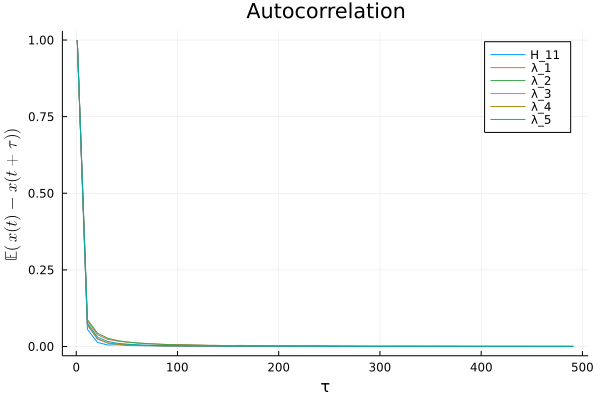
\includegraphics[width=0.5\textwidth]{autocorrelation.png}%
    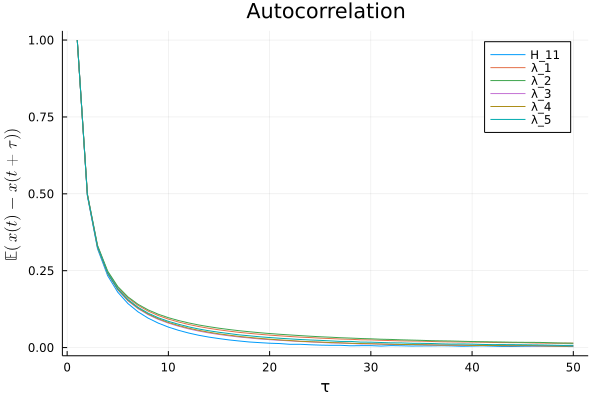
\includegraphics[width=0.5\textwidth]{autocorrelation_shortTimes.png}
  \end{figure}
\end{frame}
%%%%%%%%%%%%%%%%%%%%%%%%%%%%%%%%%%%%%%%%%%%%%%%%%%%%%%%%%%%%%%%%%%%%%%%%%%%%%

%%%%%%%%%%%%%%%%%%%%%%%%%%%%%%%%%%%%%%%%%%%%%%%%%%%%%%%%%%%%%%%%%%%%%%%%%%%%%
\begin{frame}{Comparison of invariant distributions across $Re$}
  \begin{figure}
    \centering
    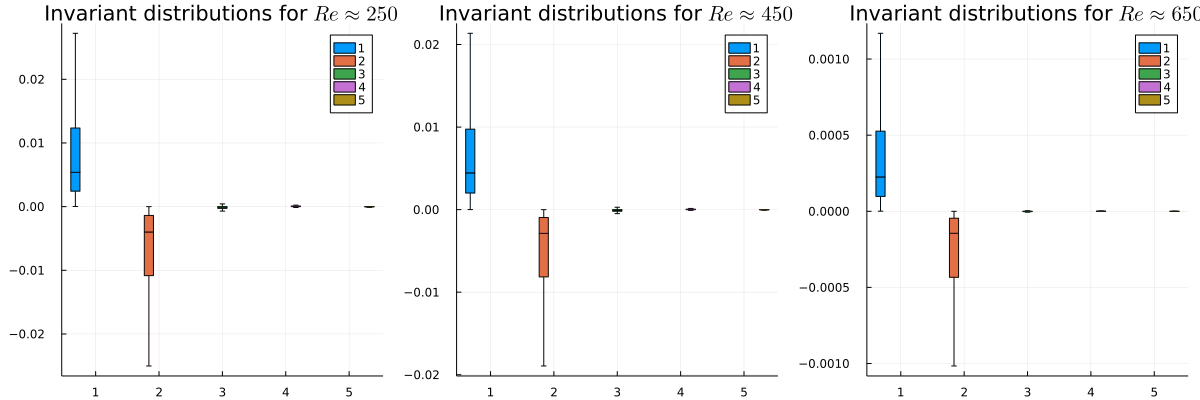
\includegraphics[width=1.0\textwidth]{invariantComparison.png}
    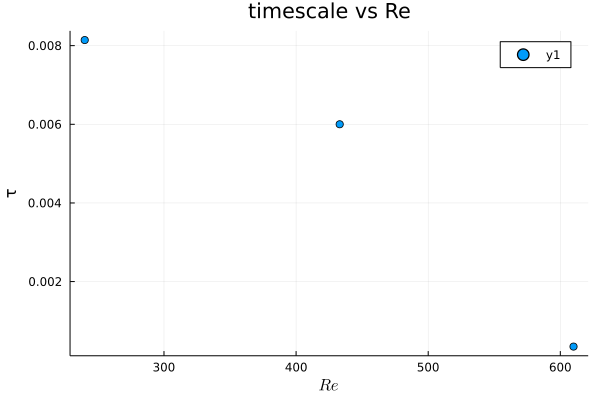
\includegraphics[width=0.5\textwidth]{timescaleVsRe.png}
  \end{figure}
  $Re \approx 240, 433, 610$
\end{frame}
%%%%%%%%%%%%%%%%%%%%%%%%%%%%%%%%%%%%%%%%%%%%%%%%%%%%%%%%%%%%%%%%%%%%%%%%%%%%%


\end{document}